\documentclass[12pt]{article}
%\usepackage{fullpage}
\usepackage{epic}
\usepackage{eepic}
\usepackage{paralist}
\usepackage{graphicx}
\usepackage{algorithm,algorithmic}
\usepackage{tikz}
\usepackage{xcolor,colortbl}
\usepackage{amsmath, amssymb}

%%%%%%%%%%%%%%%%%%%%%%%%%%%%%%%%%%%%%%%%%%%%%%%%%%%%%%%%%%%%%%%%
% This is FULLPAGE.STY by H.Partl, Version 2 as of 15 Dec 1988.
% Document Style Option to fill the paper just like Plain TeX.

\typeout{Style Option FULLPAGE Version 2 as of 15 Dec 1988}

\topmargin 0pt
\advance \topmargin by -\headheight
\advance \topmargin by -\headsep

\textheight 8.9in

\oddsidemargin 0pt
\evensidemargin \oddsidemargin
\marginparwidth 0.5in

\textwidth 6.5in
%%%%%%%%%%%%%%%%%%%%%%%%%%%%%%%%%%%%%%%%%%%%%%%%%%%%%%%%%%%%%%%%

\pagestyle{empty}
\setlength{\oddsidemargin}{0in}
\setlength{\topmargin}{-0.8in}
\setlength{\textwidth}{6.8in}
\setlength{\textheight}{9.5in}

\setcounter{secnumdepth}{0}

\setlength{\parindent}{0in}
\addtolength{\parskip}{0.2cm}
\setlength{\fboxrule}{.5mm}\setlength{\fboxsep}{1.2mm}
\newlength{\boxlength}\setlength{\boxlength}{\textwidth}
\addtolength{\boxlength}{-4mm}

\newcommand{\algosolutionbox}[2]{
  \begin{center}
    \framebox{\parbox{\boxlength}{
        \textbf{CS 5722, Fall 2014} \hfill \textbf{#1}\\
        #2
      }}
  \end{center}}

\begin{document}

\algosolutionbox{Homework 12}{
  % TODO: fill in your own name, netID, and collaborators
  Group: Michael Jalkio, Kevin Li, Daniel Sperling\\
  NetIDs: mrj77, kyl27, dhs252
}

\section{1}
\subsection{a}
See attached page.

\subsection{b}
The Pareto-Optimal set of solutions is the first three: University of Disney Land, Bedlam College and Hard Knocks U. The only school that is dominated is Space Cadet Academy, which is dominated by the University of Disney Land.

\subsection{2}

\subsubsection{a}
The following plot was produced using the NSGA II implementation in MATLAB. The weight, $f_1$ is represented on the x axis, and the deflection, $f_2$, is represented on the y axis.\\\\

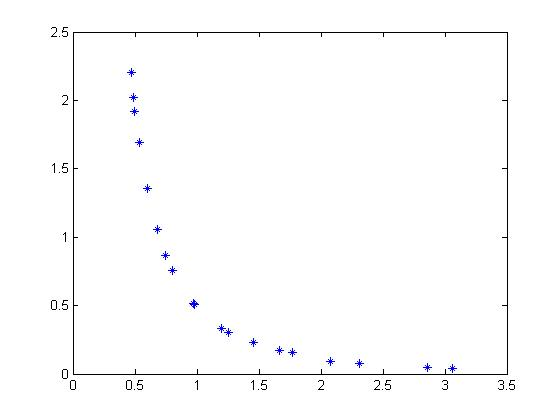
\includegraphics{pareto_optimal}

\subsubsection{b}
The mean of the weight, $f_1$, for the pareto optimal solutions is 1.3751 kg, and the standard deviation is 0.8813 kg.

\subsubsection{c}
The mean of the deflection, $f_2$, for the pareto optimal solutions is 0.7197 mm, and the standard deviation is 0.7348 mm.

\subsubsection{d}
No, we cannot say which solution is best for the problem. Since this is a multiple objective optimization problem, we don't know which solution on the pareto front may be best for the current problem, as none of them dominate the others.

\subsection{3}
\subsubsection{a}
From the graphic, we determined that there were three solutions on the first pareto front - d, 4, and 5, and four on the second pareto front, c, e, 3 and 2. To take the top 6 solutions as parents for the next round, we take every solution on the first pareto front, d, 4, and 5, and choose c, 3, and 2 from the second front, as e is the most crowded (closest to two other solutions). As such, our parents for the next round are d, 4, 5, c, 3 and 2.

\subsubsection{2}
From each pair:\\\\
c is chosen over f: Both are in the same front, but c's distance is greater.\\
2 is chosen over e: 2 is in front 1 but e is in front 2.\\
3 is chosen over 4: Both are in the same front, but 3's distance is greater.\\
f is chosen over 5: f is in front 1 but 5 is in front 2.\\
c is chosen over 3: c is in front 1 but 3 is in front 2.\\
2 is chosen over e: 2 is in front 1 but e is in fron 2. \\

\end{document}